\chapter{Concept Learning}
In this chapter we will analyze our first learning algorithm, that is not used usually in pratice but it can be useful to discover 
some aspect behind and also we will briefly introduce the effect of bias in ML model.

We define \emph{Concept Learning} as 
\begin{defi}
    Concept Learning consist in infer a boolean-valued function from training examples of its input and output
\end{defi}
It can be also formulated as a problem of searching through a predefined space of potential hypothesis for the hypothesis that best fit 
the training examples and to better introduce we consider as an example the task to discover if our friend "Aldo" enjoys his favorite water sport,
with six features (Sky, AirTemp, Humidity, Wind, Water, Forecast), as we can note in figure \ref{img:conceptExample}, and also for each attribute
the hypothesis can be "?" (every value is acceptable), a single required value and "$\emptyset$" (no value is acceptable).

\begin{figure}
    \caption{Example of EnjoySport problem}
    \label{img:conceptExample}
    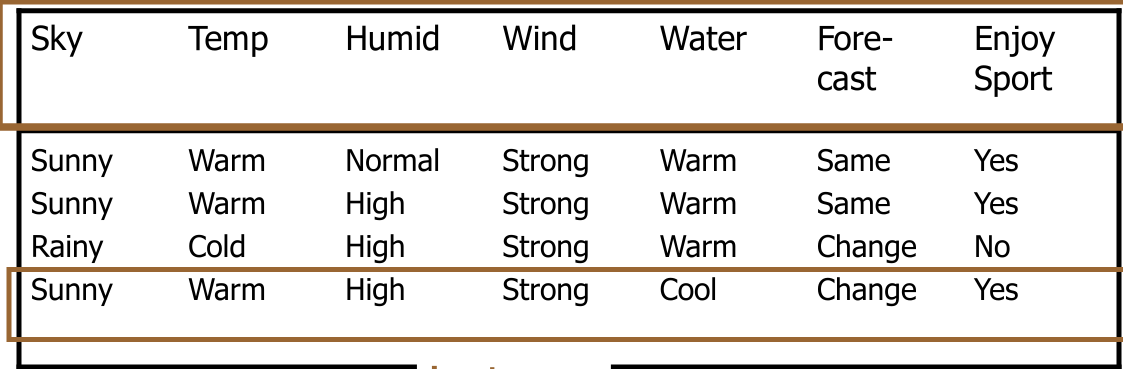
\includegraphics[width=\textwidth]{Images/enjoySport}
\end{figure}
We define now an important concept, assumpted usually in all ML models, that is important to understand and remember
\begin{defi}[Inductive Hypothesis \cite{mitchell}]
    Any hypothesis found to approximate  the target function well over a sufficiently large set of training examples will also approximate the 
    target function well over other unobserved examples.
\end{defi}
Concept Learning can be viewed as the task of searching through a large space of hypotheses implicitly defined by the hypothesis representation and 
the goal of this search is to find the hypothesis that best fits the training examples.

We define our hypothesis $h: X \to \{0, 1\}$ that satisfi4es $x$ when $h(x) = 1$ and it is consistent with our training examples $D$ if $h(x) = y \, \forall (x, y) \in D$,
so the object of concept learning is to find an hypothesis that is consistent and fits better the training examples.

Many algorithms for concept learning use a general-to-specific ordering of hypothesis to achieve a fast training, so we have
\begin{defi}
	Let $h_j$ and $h_k$ be boolean-valued functions defined over $X$, then $h_j$ is more general than or equal to $h_k (h_j \geq _G h_k)$ if and only if 
	\[ \forall x \in X h_k(x) = 1 \to h_j(x) = 1 \]
\end{defi}
Note that $\geq _G$ relation is defined independent of the target concept, they depends only on which instances satisfy the two hypothesis, and also 
this defines a partial order over the hypothesis space $H$, useful in concept learning algorithms that we will introduced and analyzed in the following paragraph.

\section{Find-S}



